\section{Tool Interactions}\label{tool-interactions}

Through the iterations described in the previous chapter, we arrived at
Foldlings' tool-based system for card design. Each tool creates a
specific type of feature --- a group of cuts and folds that define
planes that will fold together in 3D\footnote{Described in more detail
  in section \ref{interface-data-structures}, Interface Data Structures,
  on page \pageref{interface-data-structures}}. The core interaction is
as follows:

\begin{enumerate}
\def\labelenumi{\arabic{enumi}.}
\itemsep1pt\parskip0pt\parsep0pt
\item
  User selects a tool
\item
  User drags on the screen to define a feature

  \begin{enumerate}
  \def\labelenumii{\alph{enumii}.}
  \itemsep1pt\parskip0pt\parsep0pt
  \item
    (Some features require more than one touch to define)
  \end{enumerate}
\item
  The feature is added to the sketch on releasing the drag
\end{enumerate}

\subsection{Tap Options}\label{tap-options}

\begin{figure}[htbp]
\centering
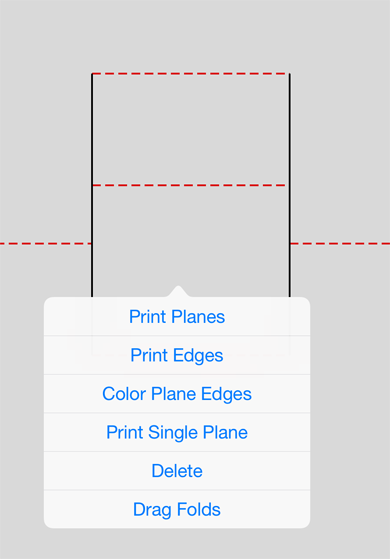
\includegraphics{figures/32_UI_Tool_Interactions/tap-options.png}
\caption{Options presented when tapping a box fold feature.}
\end{figure}

Tap options are modifications that can be made to a feature. These allow
the user to modify or delete features in the sketch. Different options
are presented based on the feature type and state. For example,
currently only leaf nodes in the feature tree have the ``Drag Folds''
option. That is, you can only move folds within a feature that has no
children. Since moving folds within a feature with children would
require modifying the folds of all of their children\footnote{Dragging
  folds in a parent feature can also cause child features to become
  invalid, depending on their fold positions.}, implementing fold
dragging in features with children is future work.

\subsection{Feature Interactions}\label{feature-interactions}

Some interactions are common to all features. To add a feature, you
select the tool that creates features of that type. Each feature
type\footnote{(Except for the master card)} has a corresponding button
in the toolbar at the bottom of the sketches. In general, all features
are defined by dragging in the drawing area. Features are generally
completed by releasing the drag. As long as you remain in that tool, you
can continue creating features of that type by dragging. Having
consistent tool interactions helps reduce the burden of learning new
tools, and allows for a scaffolded user experience.
\textbf{\textgreater{}\textgreater{}TODO cite scaffolding/play lit}

We can infer that the user has completed a sketch when a touch completes
the feature. Completion conditions are different depending on the on the
feature, but the completion state is never ambiguous. Two feature types
are always defined with a single touch: Box Fold and Free Form. The
multi-step tools --- Polygon and V Fold ---~require more than one touch
to define.

\subsubsection{Box Fold}\label{box-fold}

A box fold is created by dragging to define the bounds of the box. Box
folds are only valid if they span a driving fold.

\subsubsection{FreeForm}\label{freeform}

Free-form shapes are created by dragging a single closed shape.
Free-form shapes that cross a fold are truncated and a center fold is
automatically added at the correct height. If a free-form shape does not
cross a fold it is considered a hole, and no folds are added. Initially,
we considered having a separate tool for creating holes. However,
through informal user tests we discovered that users intuitively
understood that free-form shape that do not cross a fold will become
holes --- and therefore we were able to combine the two functions into a
single tool.

\subsubsection{Polygon}\label{polygon}

Polygons are constructed one point a time. Points are added by tapping
or dragging on the sketch, adding edges between successive points with
each tap. Once a point is (nearly) coincident with the initial point,
the feature is complete. Users can also drag existing points in the
polygon to modify the shape.

Initially, tapping was they only way to add points to a polygon --- we
added dragging points to make the interaction more consistent with other
feature types.

Polygons are the only feature that can be created by tapping rather than
dragging. This creates a conflict with tap options, which are also
accessed using a tap. If the user is in the polygon tool and taps inside
an existing feature, it is ambiguous whether they want to start a new
polygon or select a tap option. To resolve this conflict, if the first
tap of a polygon is inside another feature (besides the master card), we
display the tap options rather than creating a polygon. Users can either
start polygon within the master card or use a drag to add the first
point, if they wish to construct a polygon inside another fold feature.

\subsubsection{V-Fold}\label{v-fold}

V-Folds require two touches to complete. The first touch creates a
``vertical cut'' that crosses a fold, the second defines the point on
that fold from which diagonal folds are constructed.

\subsection{Intersecting Features}\label{intersecting-features}

Some features can be drawn over cuts and folds of existing features.
When a new feature intersects a previously-drawn feature, it occludes
existing cuts and folds --- creating the new feature on top of existing
features. The implementation of these intersections is incomplete, and
is described in \textbf{\textgreater{}\textgreater{}CITE DESCRIBED IN}

\subsection{Tutorial}\label{tutorial}

We eschewed detailed drawing instructions or a separate tutorial mode,
in favor of short video tutorials that appear the first time each tool
is used. These tutorials can also be accessed by tapping the feature
icons on the about page.

\begin{figure}[htbp]
\centering
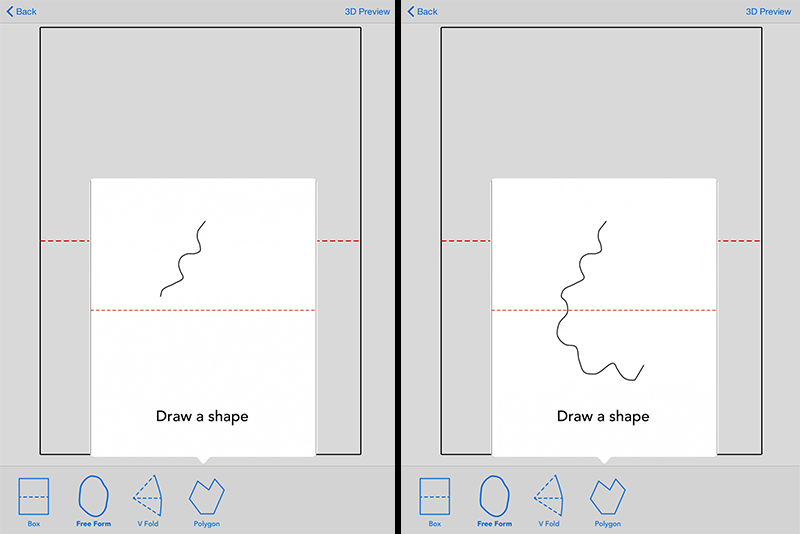
\includegraphics{figures/32_UI_Tool_Interactions/tutorial_step_one_two.png}
\caption{Free-form shape tutorial video.}
\end{figure}

We also show helpful tips between screens --- for example, when moving
to 3D preview and restoring from a saved sketch.

\subsection{Warnings and Errors}\label{warnings-and-errors}

We display warnings and errors as bright-red banners at the top of the
sketch view when. These warnings are displayed in response to failing
the validity checks performed when adding a feature to the sketch.

\begin{figure}[htbp]
\centering
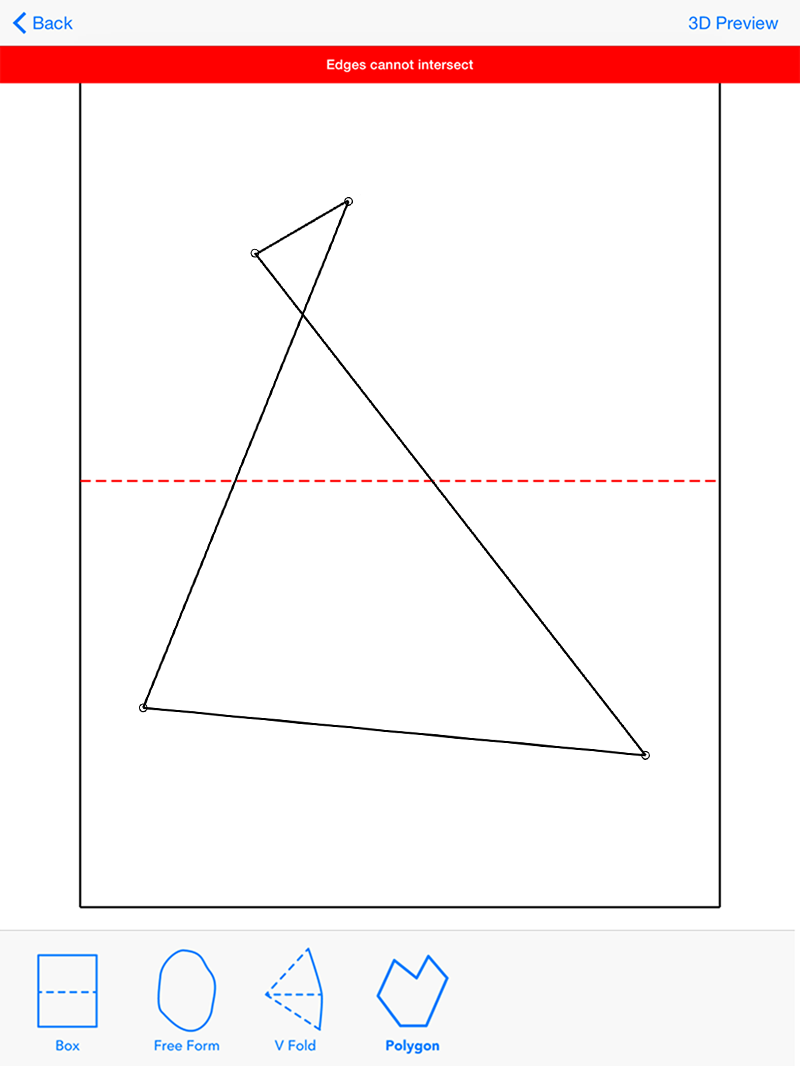
\includegraphics{figures/32_UI_Tool_Interactions/error_message.png}
\caption{An error message shown when rejecting a polygon with
intersecting edges.}
\end{figure}

The goal of these warnings is to give users descriptive feedback when
errors occur, and to give them an intuitive sense of which actions
create invalid features.

\subsection{Send to Laser Cutter}\label{send-to-laser-cutter}

In the three-dimensional preview, users can tap the ``send to laser
cutter'' option. This feature sends the user an email with an attached
SVG file. This file can be fed to a laser cutter or paper cutting
machine, or can be opened in a vector graphics editor to make further
changes.

The sketches are bound by physical constraints, as described in Chapter
X Section Y on page RAWR. \textbf{\textgreater{}\textgreater{}TODO}. One
constraint is the precision of the cutter, which limits how closely cuts
and folds can be drawn to each other. We take these physical constraints
into account during the sketching process, so the user's design is
foldable.

\subsection{Print}\label{print}

In addition to sharing an SVG file for laser cutting, users can press
``share''. This version is essentially screenshot of the 2D sketch, and
can be printed, emailed, or shared via social media. Typically, this is
the option a user would choose to cut and fold their design by hand.

\begin{figure}[htbp]
\centering
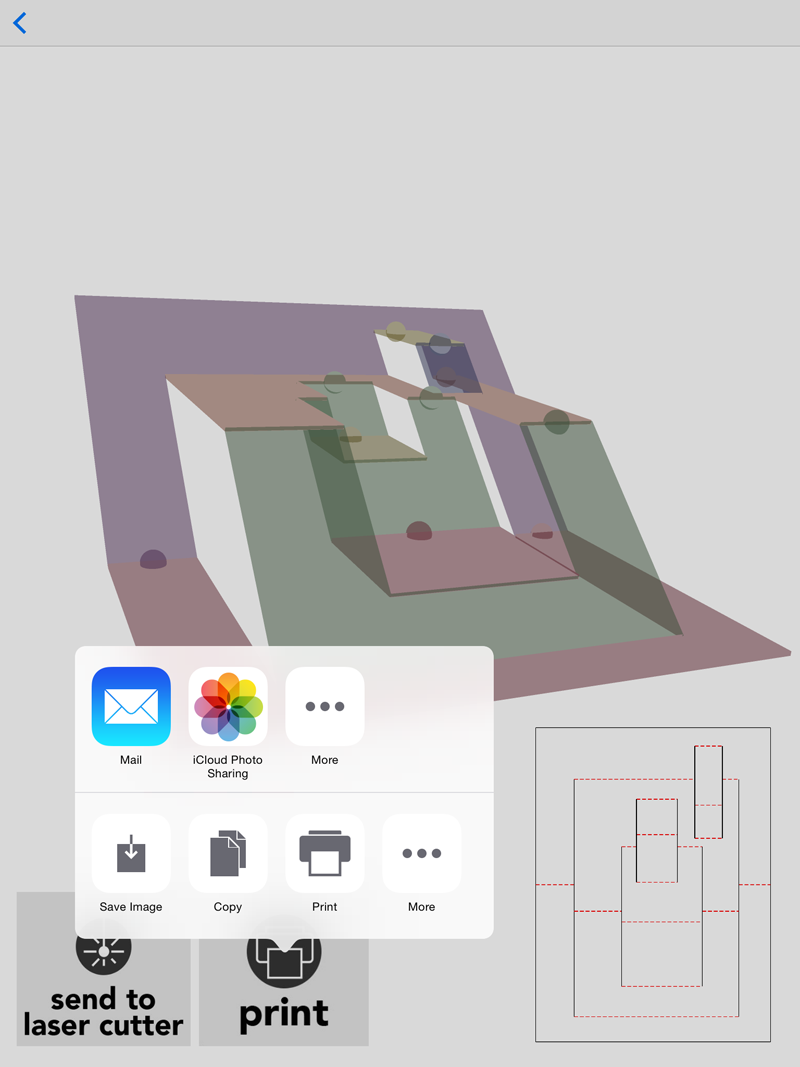
\includegraphics{figures/32_UI_Tool_Interactions/3d-share.png}
\caption{Options for sharing a fold pattern from the 3D preview.}
\end{figure}

\subsection{Visual Aids}\label{visual-aids}

\textbf{\textgreater{}\textgreater{}TODO\textgreater{}\textgreater{} ADD
FIGURE SHOWING dot vs dot-dash line}

Foldlings utility relies on the user understanding how their design will
fold while they are designing. We use visual aids to help the user.
Using data from the user study described in Chapter 3, section
\ref{visual-aids-user-study}, on page \pageref{visual-aids-user-study},
we adjusted our interface to include more cues to help users visualize
the design. The primary visual aid is the 3D preview, which displays an
interactive preview of the folded card. Users can interact with this
card through an intuitive ``pinch'' gesture. In addition, we shade
planes based on orientation (cool colors for planes that will be
vertical when the plane is halfway folded and warm colors for horizontal
planes. In the SVG file (accessed via ``send to laser cutter''), we
adjust line dash patterns for folds based on orientation: dotted lines
are mountains, creased away from the main fold --- dot-dash lines are
valleys, creased in the same direction as the main fold. From the visual
aids user study, we ~have data that suggest showing fold orientation is
very helpful to users folding cards.

\begin{figure}[htbp]
\centering
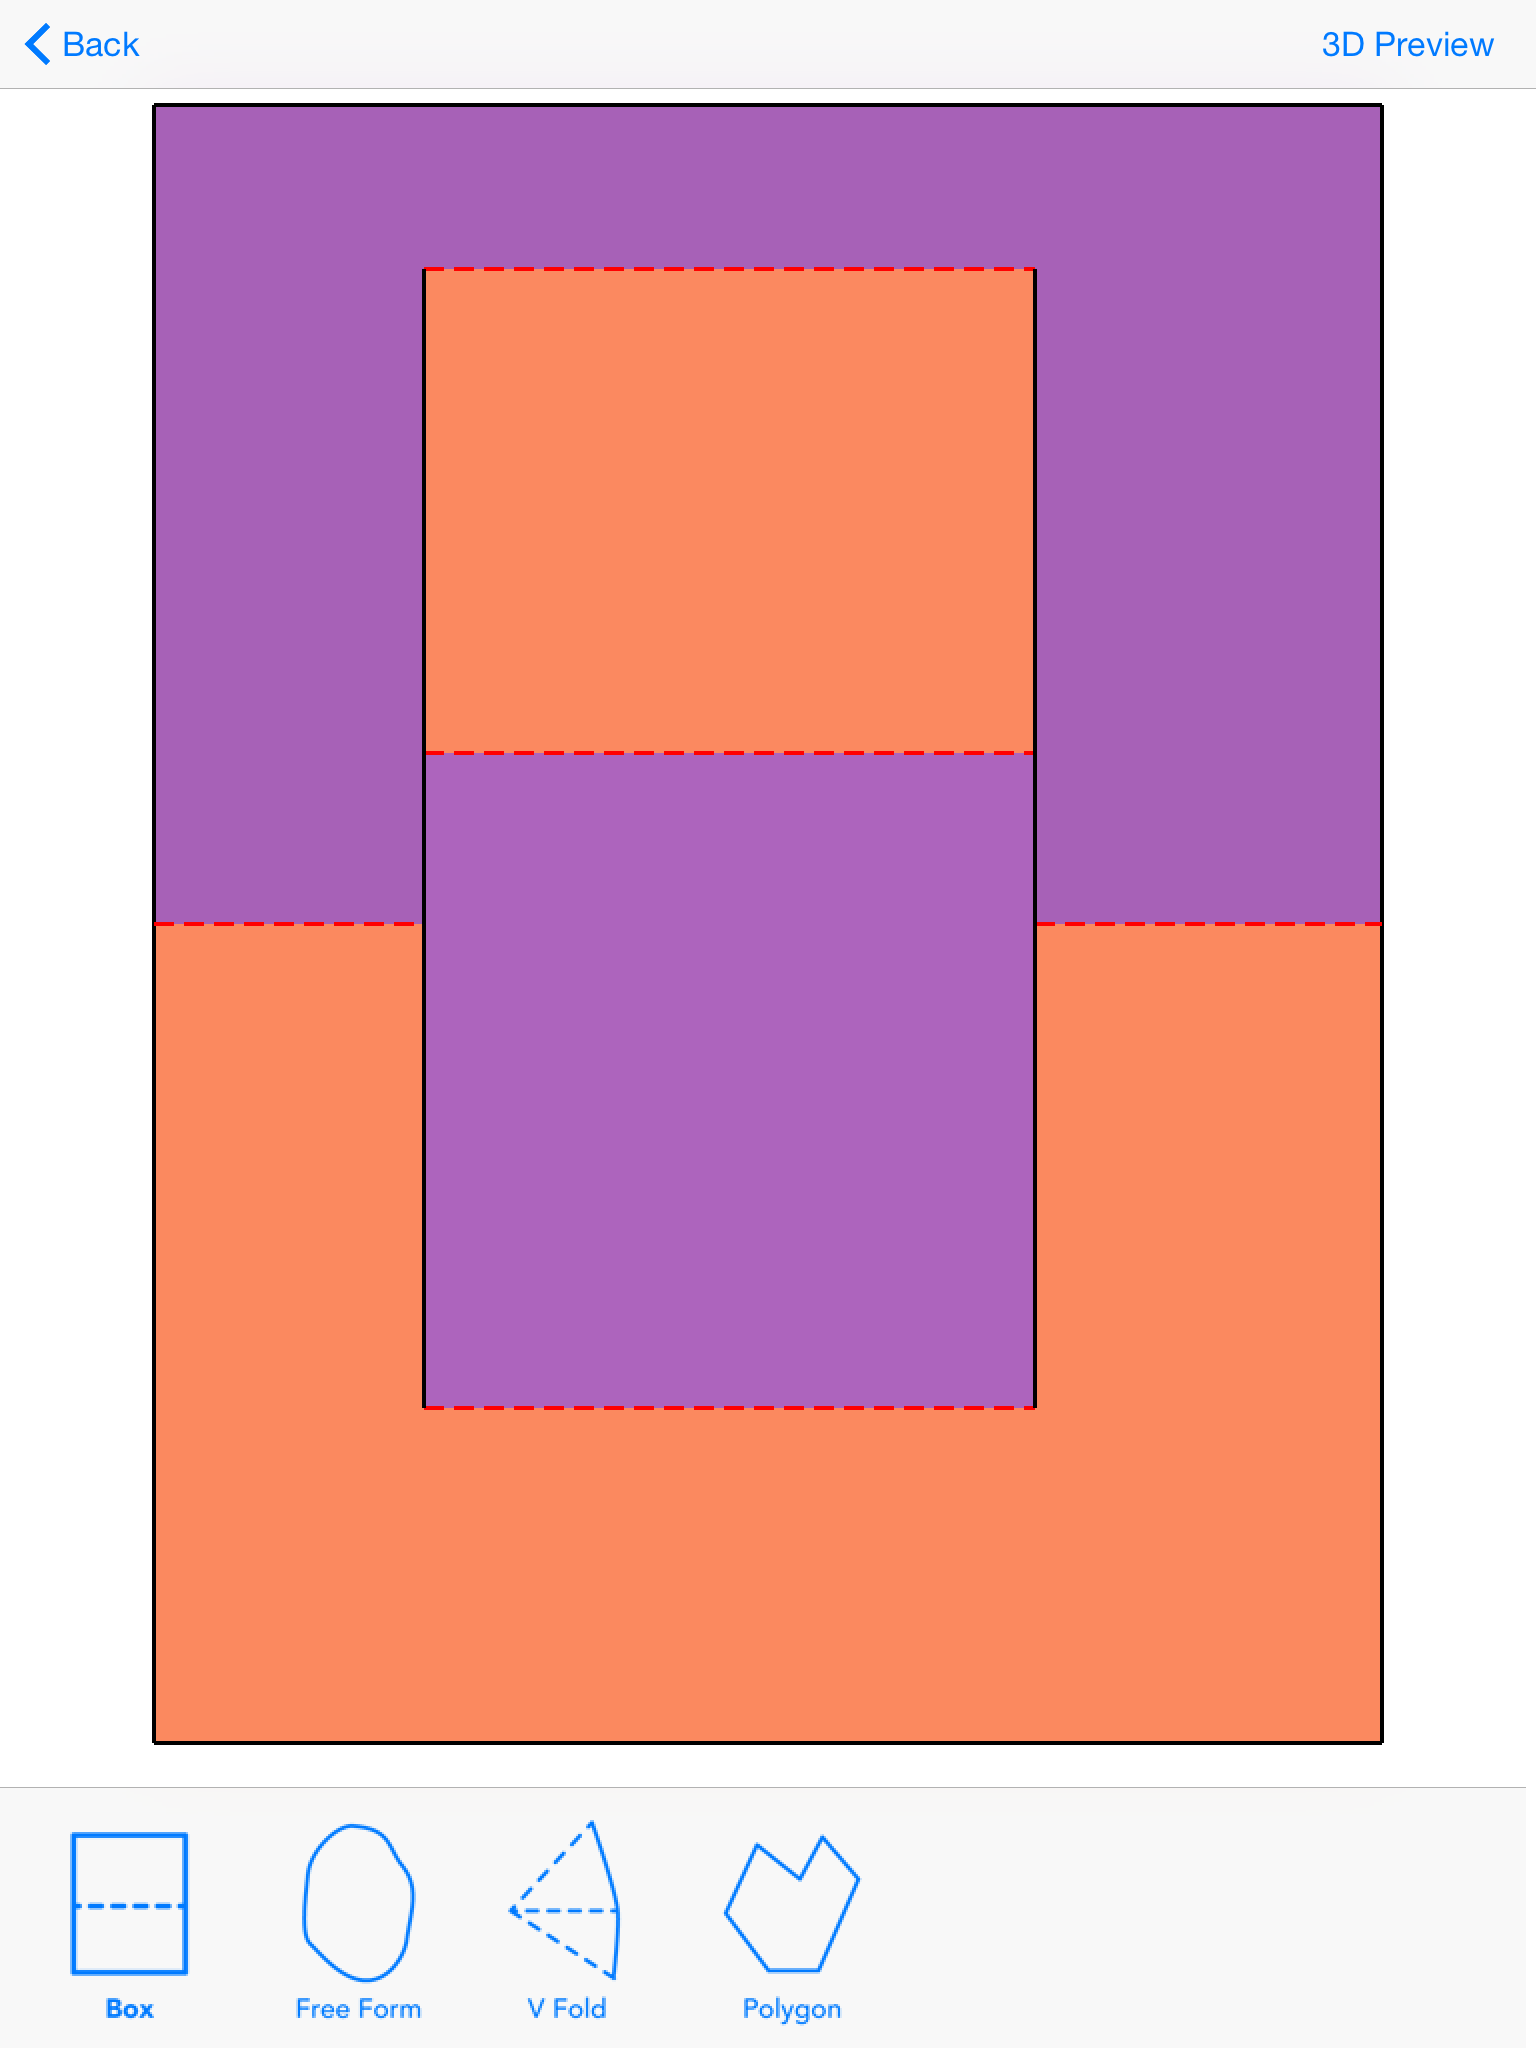
\includegraphics{figures/32_UI_Tool_Interactions/currentInterface.png}
\caption{Plane shading is one of many visual aids in Foldlings.}
\end{figure}
